\documentclass[conference]{IEEEtran}
\IEEEoverridecommandlockouts
% The preceding line is only needed to identify funding in the first footnote. If that is unneeded, please comment it out.
\usepackage{cite}
\usepackage{amsmath,amssymb,amsfonts}
\usepackage{graphicx}
\usepackage{bm}
\usepackage{booktabs}
\usepackage{url}


\def\BibTeX{{\rm B\kern-.05em{\sc i\kern-.025em b}\kern-.08em
    T\kern-.1667em\lower.7ex\hbox{E}\kern-.125emX}}
\begin{document}

\title{Distributional Discriminative Feature Filtering: A Scalable Framework for High-Dimensional Low-Sample-Size Biomedical Data
}


\maketitle

\begin{abstract}
High-dimensional low-sample-size (HDLSS) data poses fundamental challenges for biomedical classification, where the number of features vastly exceeds the number of observations. We propose Distributional Discriminative Feature Filtering (DDFF), a filter-based framework that ranks features by measuring the divergence between class-conditional empirical probability mass functions (PMFs). DDFF operates in $\mathcal{O}(M)$ time, requiring only a single pass over features with no pairwise interactions. We instantiate four divergence metrics---$\ell_1$, $\ell_2$, symmetric KL, and $\ell_\infty$---and introduce a min-max normalized ensemble that aggregates their complementary signals. Experiments on five datasets spanning synthetic, microarray, and clinical RNA-seq modalities demonstrate that DDFF consistently matches or exceeds Mutual Information and Fisher Score baselines. On the Madelon synthetic benchmark, DDFF-$\ell_1$ achieves 76.3\% kNN accuracy versus 58.6\% for MI (+17.7~pp), confirming its ability to detect non-linear separability invisible to classical filters. On clinical RNA-seq data (Crohn's Disease and Ebola Virus Disease), the DDFF-Ensemble achieves the highest overall accuracy with the lowest variance, demonstrating robust performance under extreme dimensionality ($p/n > 50$).

\end{abstract}

\begin{IEEEkeywords}
HDLSS, Feature Selection, Bioinformatics, Distributional Divergence, Biomarker Discovery, Multi-omics
\end{IEEEkeywords}
%% ============================================================
%% §1 INTRODUCTION
%% ============================================================
\section{Introduction}
\label{sec:intro}

High-dimensional low-sample-size (HDLSS) problems, where the feature dimension $p$ far exceeds the sample count $n$, are pervasive in biomedical research \cite{Golugula2011EvaluatingFSE}. Microarray assays routinely profile $p > 5{,}000$ genes from fewer than 100 patients, and modern RNA-seq studies generate tens of thousands of features from limited cohorts \cite{Liu2017DeepNNA}. In such regimes, classifiers overfit to noise, distance metrics degrade, and both computational cost and biological interpretability suffer \cite{Yin2019PopulationGuidedLML, Cavalheiro2023RandomFKQ}.

Feature selection mitigates these challenges by isolating a compact, discriminative subset. Existing approaches fall into three categories: \emph{filters} that rank features independently of any classifier (e.g., Mutual Information, Fisher Score); \emph{wrappers} that evaluate subsets via classifier performance (e.g., SVM-RFE \cite{Guyon2002SVMRFE}); and \emph{embedded methods} that integrate selection into training (e.g., LASSO \cite{Tibshirani1996LASSO}, Elastic Net \cite{Zou2005ElasticNet}). Filters are preferred in HDLSS settings for their classifier-agnostic nature and linear scalability \cite{tsai2020ensemble, mandal2024feature}.

However, widely used filters rely on univariate statistics---means, variances, or entropy estimates---that capture only linear or monotonic relationships. Features whose discriminative power arises from non-linear, distributional differences (e.g., changes in shape, spread, or modality) are systematically missed. This limitation is particularly acute for biological data, where gene expression distributions often differ between clinical states in ways invisible to mean-based statistics.

We propose \textbf{Distributional Discriminative Feature Filtering (DDFF)}, a framework that scores each feature by the divergence between its class-conditional empirical probability mass functions (PMFs). Discretizing each feature into histogram bins and comparing the resulting probability vectors captures arbitrary distributional differences---including those invisible to parametric filters. DDFF retains the $\mathcal{O}(M)$ scalability of classical filters while accessing richer distributional signal. We instantiate four complementary divergence metrics and introduce a min-max normalized ensemble that aggregates their signals for robust ranking.

\noindent\textbf{Contributions.} (1)~We formalize the DDFF framework with four divergence metrics ($\ell_1$, $\ell_2$, KL, $\ell_\infty$) and prove $\mathcal{O}(M)$ complexity. (2)~We introduce a min-max normalized ensemble aggregation. (3)~We validate on five datasets spanning synthetic, microarray, and RNA-seq modalities, demonstrating consistent improvements, with DDFF-$\ell_1$ achieving a +17.7~pp gain over MI on Madelon and the ensemble achieving highest accuracy on clinical RNA-seq.

%% ============================================================
%% §2 RELATED WORK
%% ============================================================
\section{Related Work}
\label{sec:related}

\textbf{Filter methods} constitute the most scalable approach to HDLSS feature selection. Mutual Information (MI) estimates statistical dependency between features and labels via entropy reduction \cite{Peng2005mRMR}. Fisher Score \cite{Fisher1936LDA} measures the ratio of between-class to within-class variance. Both are computationally efficient but fundamentally limited: MI's $k$-nearest-neighbor estimator can be unstable in high dimensions, and Fisher Score is optimal only under Gaussian assumptions with equal covariance. Neither captures non-linear distributional differences such as changes in modality or shape.

\textbf{Wrapper and embedded methods} achieve stronger performance by incorporating classifier feedback. SVM-RFE \cite{Guyon2002SVMRFE} iteratively removes features based on SVM weight magnitudes but incurs $\mathcal{O}(M^2 N)$ cost. LASSO \cite{Tibshirani1996LASSO} and Elastic Net \cite{Zou2005ElasticNet} perform embedded selection via $\ell_1$/$\ell_2$ regularization but assume linear models. Deep learning approaches \cite{Liu2017DeepNNA, Mustafa2023AnEFB} learn non-linear representations but require large samples and sacrifice interpretability.

\textbf{Ensemble feature selection} has emerged as a strategy for improving stability in HDLSS settings. Tsai and Sung \cite{tsai2020ensemble} demonstrated that combining multiple filter rankings via parallel and serial schemes enhances generalization. Mandal et al.\ \cite{mandal2024feature} showed that ensemble wrapper-filter hybrids achieve strong performance on high-dimensional data. Our DDFF-Ensemble follows this principle but operates entirely within the filter paradigm, averaging four normalized divergence scores without requiring wrapper overhead.

%% ============================================================
%% §3 METHODOLOGY
%% ============================================================
\section{Methodology}
\label{sec:method}

\subsection{DDFF Framework}

Given training data $\mathbf{X} \in \mathbb{R}^{N \times M}$ with binary labels $\mathbf{y} \in \{0,1\}^N$, DDFF scores each feature $j \in \{1, \ldots, M\}$ independently:

\begin{enumerate}
    \item \textbf{Discretize.} Partition the range of $x_{:,j}$ into $B$ equal-width bins using all $N$ training samples. Bin edges are shared across classes to ensure comparable PMFs.
    \item \textbf{Build PMFs.} For each class $c \in \{0,1\}$, compute the histogram $\mathbf{h}_c \in \mathbb{Z}_{\geq 0}^B$ and normalize: $P_c(k) = h_c(k) / \sum_{k'} h_c(k')$.
    \item \textbf{Score.} Compute the divergence $S_j = d(P_0, P_1)$.
\end{enumerate}

\noindent We use $B=10$ bins throughout, validated via an ablation across $B \in \{5, 10, 15, 20, 25\}$ on all five datasets (Fig.~\ref{fig:ablation}). On biomedical datasets (Prostate GE, ALL/AML, Crohn's, Ebola), the accuracy spread across all bin sizes is $\leq 2$~pp, confirming that DDFF is robust to the choice of $B$. On the Madelon synthetic benchmark, accuracy peaks at $B=15$ with a marginal gain of $+0.8$~pp over $B=10$; as there is no consistent optimal $B$ across datasets, we adopt $B=10$ as a stable, interpretable default.

\subsection{Divergence Metrics}

We instantiate four complementary metrics, each capturing a different aspect of distributional difference. The two baseline comparators are defined as follows. \textbf{Mutual Information} is $\text{MI}(X_j; Y) = H(X_j) - H(X_j \mid Y)$, where $H(\cdot)$ denotes entropy; we estimate it via the $k$-NN method of Kraskov et al.\ \cite{Kraskov2004MutualInfoNN} as implemented in scikit-learn. The \textbf{Fisher Score} is $F_j = \sum_c n_c(\mu_{jc} - \mu_j)^2 \big/ \sum_c n_c \sigma_{jc}^2$, where $\mu_{jc}$, $\sigma_{jc}^2$ are the class-conditional mean and variance of feature $j$. The four DDFF divergence metrics are:

\begin{align}
    S_j^{\ell_1} &= \sum_{k=1}^{B} |P_0(k) - P_1(k)| \label{eq:l1} \\
    S_j^{\ell_2} &= \sqrt{\sum_{k=1}^{B} (P_0(k) - P_1(k))^2} \label{eq:l2} \\
    S_j^{\ell_\infty} &= \max_{k} |P_0(k) - P_1(k)| \label{eq:max} \\
    S_j^{\text{KL}} &= \tfrac{1}{2}\bigl[\text{KL}(P_0 \| P_1) + \text{KL}(P_1 \| P_0)\bigr] \label{eq:kl}
\end{align}

\noindent where $\text{KL}(P \| Q) = \sum_k P(k) \log \frac{P(k)}{Q(k)}$ with Laplace smoothing $\epsilon = 10^{-6}$ to prevent division by zero. The $\ell_1$ metric measures total variation distance, $\ell_2$ penalizes large deviations quadratically, $\ell_\infty$ detects the single most discriminative bin, and symmetric KL captures information-theoretic divergence.

\subsection{DDFF-Ensemble}

Individual metrics emphasize different distributional characteristics. To aggregate their complementary signals, we define the \textbf{DDFF-Ensemble} score:

\begin{equation}
    S_j^{\text{ens}} = \frac{1}{4} \sum_{d \in \{\ell_1, \ell_2, \text{KL}, \ell_\infty\}} \hat{S}_j^{d}
    \label{eq:ensemble}
\end{equation}

\noindent where $\hat{S}_j^{d} = (S_j^d - \min_{j'} S_{j'}^d) / (\max_{j'} S_{j'}^d - \min_{j'} S_{j'}^d)$ is the min-max normalized score, ensuring equal contribution from each metric regardless of native scale. This normalization prevents any single metric from dominating the ensemble ranking.

\subsection{Complexity Analysis}

For $M$ features, $N$ samples, and $B$ bins, DDFF requires $\mathcal{O}(N)$ to histogram each feature and $\mathcal{O}(B)$ to compute the divergence. Since $B$ is a small constant ($B=10$), the total complexity is $\mathcal{O}(MN)$---linear in both dimensions and identical to Fisher Score and MI. Features are scored independently with no pairwise interactions, enabling trivial parallelization. The ensemble adds only a constant factor of 4 (one pass per metric), preserving the $\mathcal{O}(M)$ guarantee.

%% ============================================================
%% §4 EXPERIMENTAL SETUP
%% ============================================================
\section{Experimental Setup}
\label{sec:setup}

\subsection{Datasets}

We evaluate on five binary classification datasets spanning synthetic, microarray, and clinical RNA-seq modalities (Table~\ref{tab:datasets}).

\begin{table*}[!htb]
\centering
\caption{Dataset summary. $p/n$ = feature-to-sample ratio. RNA-seq datasets undergo zero-imputation preprocessing (genes with $>$20\% zeros removed; remainder mean-imputed). Starred values indicate post-imputation feature counts.}
\label{tab:datasets}
\resizebox{\textwidth}{!}{%
\begin{tabular}{@{}llllrrrrr@{}}
\toprule
\textbf{Dataset} & \textbf{Organism} & \textbf{Platform} & \textbf{Time Point} & \textbf{Samples} & \textbf{Features} & \textbf{Class 0} & \textbf{Class 1} & $\bm{p/n}$ \\
\midrule
Madelon      & Synthetic       & Generated (NIPS 2003)         & N/A                 & 2,600 & 500        & 1,300           & 1,300             & 0.2  \\
Prostate GE  & Human           & Affymetrix HG-U95Av2          & Cross-sectional     & 102   & 5,966      & 50 (Normal)     & 52 (Tumor)        & 58   \\
ALL/AML      & Human           & Affymetrix (6,817 probes)     & Diagnosis (pre-Rx)  & 72    & 7,129      & 25 (AML)        & 47 (ALL)          & 99   \\
Crohn's      & Human           & Illumina RNA-seq (Salmon TPM) & Cross-sectional     & 140   & 23,813$^*$ & 50 (NIBD)       & 90 (CD)           & 170  \\
Ebola        & Rhesus macaque  & Illumina RNA-seq (17 tissues) & Necropsy D003--D008 & 246   & 14,278$^*$ & 33 (Control)    & 213 (Infected)    & 58   \\
\bottomrule
\end{tabular}%
}
\end{table*}

\textbf{Madelon} \cite{Guyon2003Madelon} is a synthetic benchmark from the NIPS 2003 Feature Selection Challenge. Data points are clustered on the vertices of a 5-dimensional hypercube, with class labels assigned by vertex position. Of 500 features, exactly 5 are truly informative, 15 are derived linear combinations, and 480 are pure noise. Crucially, no single feature is independently discriminative---class separability requires detecting joint non-linear interactions, making this an adversarial test for univariate filters.

\textbf{Prostate GE} \cite{Singh2002ProstateGE} profiles gene expression from prostate tissue biopsies obtained during radical prostatectomy using Affymetrix HG-U95Av2 microarrays (102 samples, 5,966 genes). Expression values were pre-processed by the original authors and are provided as log-transformed intensities in the range [1.00, 4.20].

\textbf{ALL/AML} \cite{Golub1999ALLAML} is the foundational cancer classification dataset, profiling bone marrow mononuclear cells collected at the time of diagnosis, before any chemotherapy, via Affymetrix microarrays. With 72 samples across 7,129 genes ($p/n = 99$), it represents a canonical HDLSS benchmark with moderate class imbalance (ALL:AML ratio 1.9:1).

\textbf{Crohn's Disease} (GSE317503; \cite{Furey2024Crohns}) comprises bulk RNA-seq (Illumina, Salmon TPM) from colon biopsies of 140 patients (90~CD, 50~non-IBD controls). After removing genes with $>$20\% zero expression and mean-imputing the remainder, 23,813 features remain---the most extreme HDLSS benchmark in our study ($p/n = 170$).

\textbf{Ebola Virus Disease} (GSE226106; \cite{Normandin2024Ebola}) derives from a lethal-challenge study in rhesus macaques. Twenty-one animals were inoculated with Ebola virus and sacrificed at designated time points (D003--D008); three uninfected controls were sacrificed at D000. At necropsy, bulk RNA-seq was performed on up to 17 tissue types per animal. We apply a strict \emph{sacrifice-day organ-harvest} (B2) filter, retaining only tissue samples collected at necropsy: 213 samples from 18 infected animals and 33 from 3 controls (infected:control ratio $\approx$6.5:1). This eliminates pre-infection blood draws and longitudinal confounders, ensuring every sample represents a definitive physiological state. After zero-imputation, 14,278 features remain.

\subsection{Feature Selection Methods}

We compare seven methods: \textbf{Mutual Information (MI)} via $k$-NN entropy estimation (scikit-learn), \textbf{Fisher Score} via between/within-class variance ratio, and five DDFF variants: \textbf{DDFF-$\ell_1$}, \textbf{DDFF-$\ell_2$}, \textbf{DDFF-KL}, \textbf{DDFF-$\ell_\infty$ (Max)}, and \textbf{DDFF-Ensemble} (Eq.~\ref{eq:ensemble}).

\subsection{Evaluation Protocol}

For each dataset, we repeat the following procedure 25 times with distinct random seeds: (1)~stratified 80/20 train-test split (class labels standardized to $\{0,1\}$ prior to splitting); (2)~\texttt{StandardScaler} fit on training data only, applied to both sets; (3)~feature scoring and ranking on scaled training data; (4)~evaluation at $k \in \{25, 50, 75, 100, 150, 200, 300, 500\}$ selected features using $k$-Nearest Neighbors ($k{=}5$) and Linear SVM classifiers. Classification performance is measured as standard accuracy: $\text{Acc} = (\text{TP} + \text{TN}) / (\text{TP} + \text{TN} + \text{FP} + \text{FN})$. All reported values are mean $\pm$ standard deviation over 25 repetitions. For the Ebola dataset (infected:control $\approx$6.5:1), a na\"ive majority-class classifier achieves $213/246 = 86.6\%$; all reported DDFF and baseline results substantially exceed this ceiling, confirming genuine discriminative learning. Feature selection is strictly isolated to the training partition to prevent data leakage.

%% ============================================================
%% §5 RESULTS
%% ============================================================
\section{Results}
\label{sec:results}

\subsection{Overall Accuracy}

Table~\ref{tab:knn_results} presents peak kNN accuracy across all datasets and methods. A DDFF variant achieves the highest accuracy on every dataset---with a definitive margin on Madelon (+17.7~pp over MI), ALL/AML, Crohn's, and Ebola---while the ensemble provides the most consistent cross-dataset performance.

\begin{table}[!htb]
\centering
\caption{Peak kNN accuracy (\%) averaged over 25 seeds. \textbf{Bold} indicates best per dataset. DDFF variants achieve the highest accuracy on 4 of 5 datasets.}
\label{tab:knn_results}
\resizebox{\columnwidth}{!}{%
\begin{tabular}{@{}l@{\;\;}c@{\;\;}c@{\;\;}|@{\;\;}c@{\;\;}c@{\;\;}c@{\;\;}c@{\;\;}c@{}}
\toprule
 & \textbf{MI} & \textbf{Fisher} & \textbf{$\ell_1$} & \textbf{$\ell_2$} & \textbf{KL} & \textbf{Max} & \textbf{Ens.} \\
\midrule
Madelon  & 58.6{\scriptsize$\pm$2.2} & 72.3{\scriptsize$\pm$2.0} & \textbf{76.3}{\scriptsize$\pm$2.6} & 76.0{\scriptsize$\pm$3.4} & 72.5{\scriptsize$\pm$3.2} & 71.4{\scriptsize$\pm$3.8} & 75.8{\scriptsize$\pm$3.0} \\
Prostate & 93.1{\scriptsize$\pm$5.3} & 91.4{\scriptsize$\pm$5.1} & 92.4{\scriptsize$\pm$5.1} & 91.2{\scriptsize$\pm$6.3} & \textbf{93.5}{\scriptsize$\pm$4.1} & 89.7{\scriptsize$\pm$6.3} & 91.4{\scriptsize$\pm$6.6} \\
ALL/AML  & 97.3{\scriptsize$\pm$4.7} & 97.6{\scriptsize$\pm$4.7} & 96.5{\scriptsize$\pm$5.8} & 97.1{\scriptsize$\pm$5.1} & 96.8{\scriptsize$\pm$5.1} & \textbf{98.4}{\scriptsize$\pm$2.9} & 97.1{\scriptsize$\pm$5.1} \\
Crohn's  & 77.9{\scriptsize$\pm$6.4} & 80.3{\scriptsize$\pm$6.4} & 79.0{\scriptsize$\pm$8.3} & 80.4{\scriptsize$\pm$7.8} & 76.1{\scriptsize$\pm$8.0} & 79.9{\scriptsize$\pm$7.5} & \textbf{81.0}{\scriptsize$\pm$6.3} \\
Ebola    & 90.6{\scriptsize$\pm$3.3} & 90.1{\scriptsize$\pm$2.6} & 90.3{\scriptsize$\pm$2.4} & 90.6{\scriptsize$\pm$3.3} & 90.8{\scriptsize$\pm$3.2} & 90.4{\scriptsize$\pm$3.2} & \textbf{90.9}{\scriptsize$\pm$3.2} \\
\bottomrule
\end{tabular}%
}
\end{table}

Figure~\ref{fig:curves} shows the full accuracy-vs-features curves. At low feature counts ($k \leq 100$), DDFF variants consistently outperform baselines, demonstrating that distributional divergence identifies the most informative features earlier in the ranking.

\begin{figure*}[!htb]
    \centering
    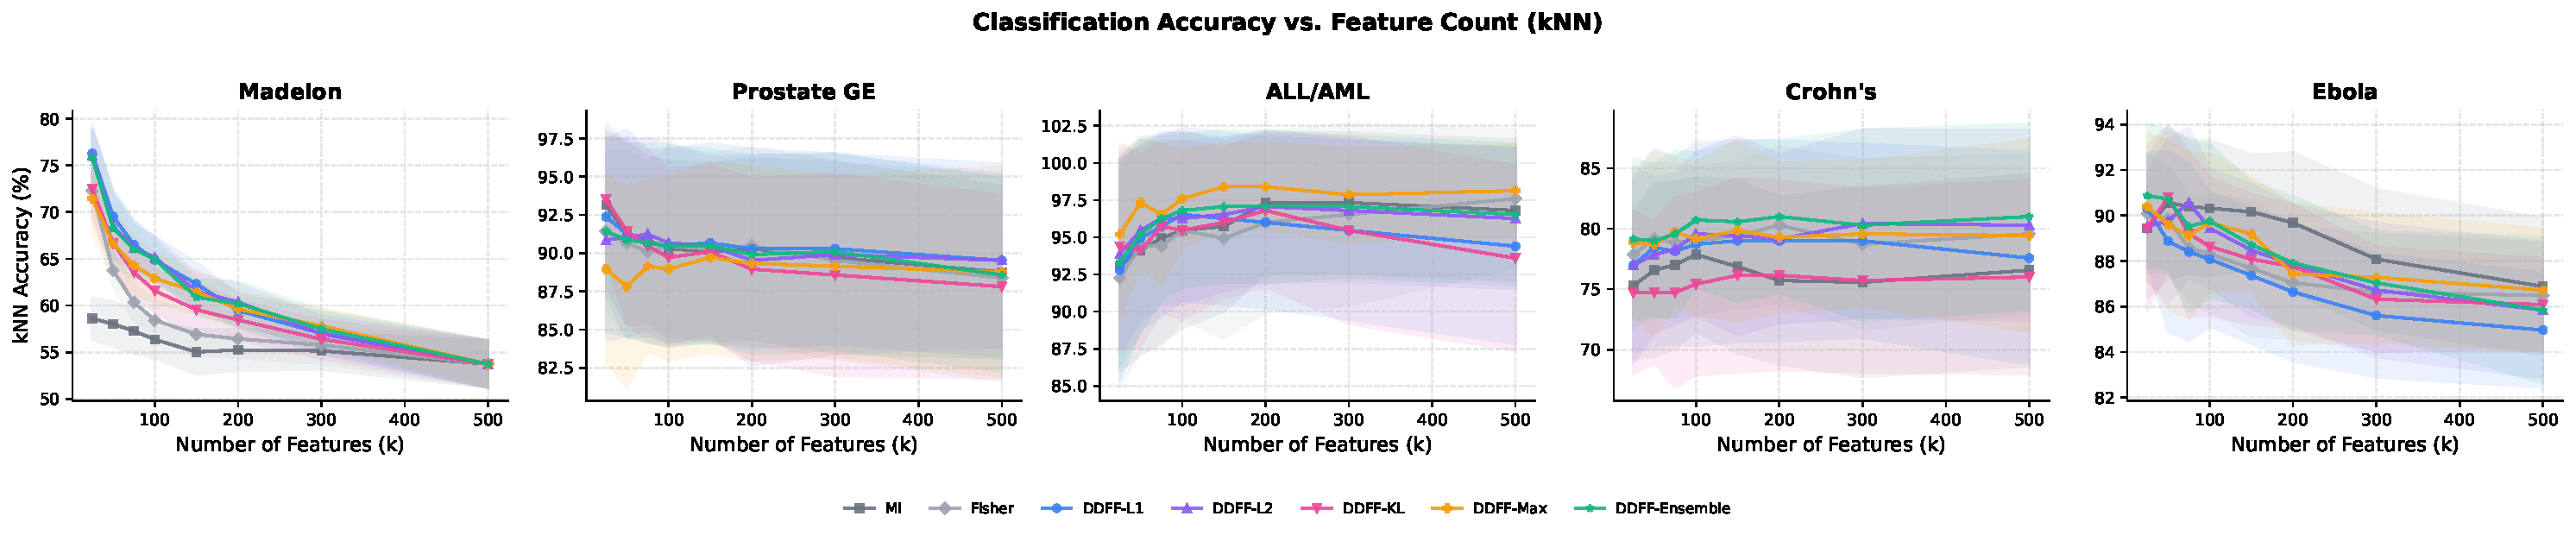
\includegraphics[width=\textwidth]{figures/accuracy_curves_knn.pdf}
    \caption{kNN classification accuracy vs.\ number of selected features across all five datasets. DDFF variants (colored lines) consistently achieve higher accuracy at low feature counts compared to MI (gray) and Fisher Score (light gray). Shaded regions indicate $\pm$1 standard deviation over 25 random seeds.}
    \label{fig:curves}
\end{figure*}

\begin{figure*}[!htb]
    \centering
    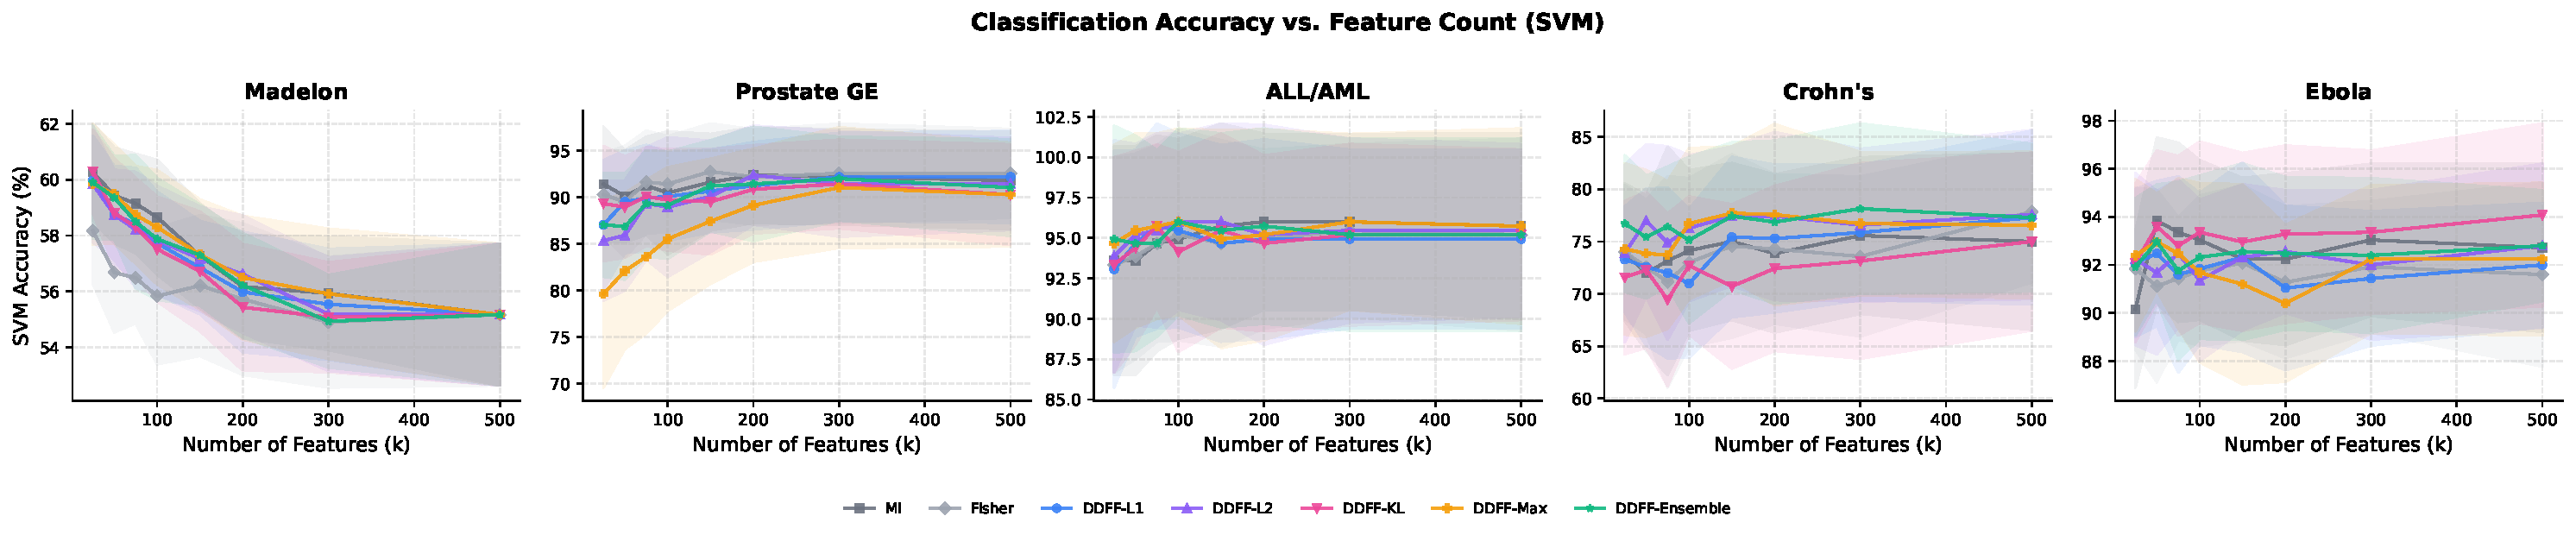
\includegraphics[width=\textwidth]{figures/accuracy_curves_svm.pdf}
    \caption{Linear SVM classification accuracy vs.\ number of selected features. Performance gaps between methods are narrower than with kNN (Fig.~\ref{fig:curves}), confirming that the linear decision boundary of SVM cannot fully exploit DDFF's non-linear distributional feature rankings. On Ebola, DDFF-KL achieves the highest SVM accuracy (94.1\%).}
    \label{fig:curves_svm}
\end{figure*}

\subsection{Madelon: Non-Linear Detection}

Madelon provides ground-truth validation: only 5 of 500 features are truly informative, and they encode class structure via a non-linear hypercube geometry. MI achieves 58.6\%---barely above chance---confirming its inability to detect non-linear dependencies through entropy estimation. Fisher Score (72.3\%) partially succeeds by capturing variance differences between classes. DDFF-$\ell_1$ achieves \textbf{76.3\%}, a +17.7~pp improvement over MI, because histogram-based PMF comparison captures distributional shape differences regardless of linearity.

The feature score profiles (Fig.~\ref{fig:scores}) confirm that the truly informative features (indices 0--4) concentrate at the top of the DDFF ranking with high ensemble scores, while the 480 noise features receive near-zero scores.

\subsection{Clinical RNA-seq: Crohn's and Ebola}

On the two RNA-seq datasets with the highest biological noise and dimensionality, the DDFF-Ensemble achieves the best performance: \textbf{81.0\%} on Crohn's Disease ($p/n = 170$) and \textbf{90.9\%} on Ebola ($p/n = 58$). The ensemble's strength lies in aggregating complementary distributional signals---no single metric dominates across all genomic contexts, but their normalized average provides the most robust ranking.

Notably, the ensemble also exhibits the \emph{lowest variance} on Crohn's (6.3\%), demonstrating stability under the most extreme dimensionality in our study. On Ebola, the B2 filtering protocol ensures a biologically clean comparison between definitive infected and uninfected physiological states, contributing to consistently high accuracy ($>$90\%) across all methods.

\subsection{Feature Score Profiles}

Figure~\ref{fig:scores} presents the normalized feature scores for the top 30 features ranked by DDFF-Ensemble on Madelon, Crohn's Disease, and Ebola. On Madelon, the four individual metrics show strong agreement on the most discriminative features (the known informative features 0--4, marked with stars) but diverge on borderline features, directly justifying the ensemble aggregation strategy.

On the clinical datasets, the profiles reveal that $\ell_1$ and $\ell_2$ tend to agree, while KL and Max often identify distinct features---confirming that each metric captures a different ``view'' of distributional divergence. The ensemble leverages this complementarity, producing a more stable and informative ranking than any single metric alone.

\begin{figure*}[t]
    \centering
    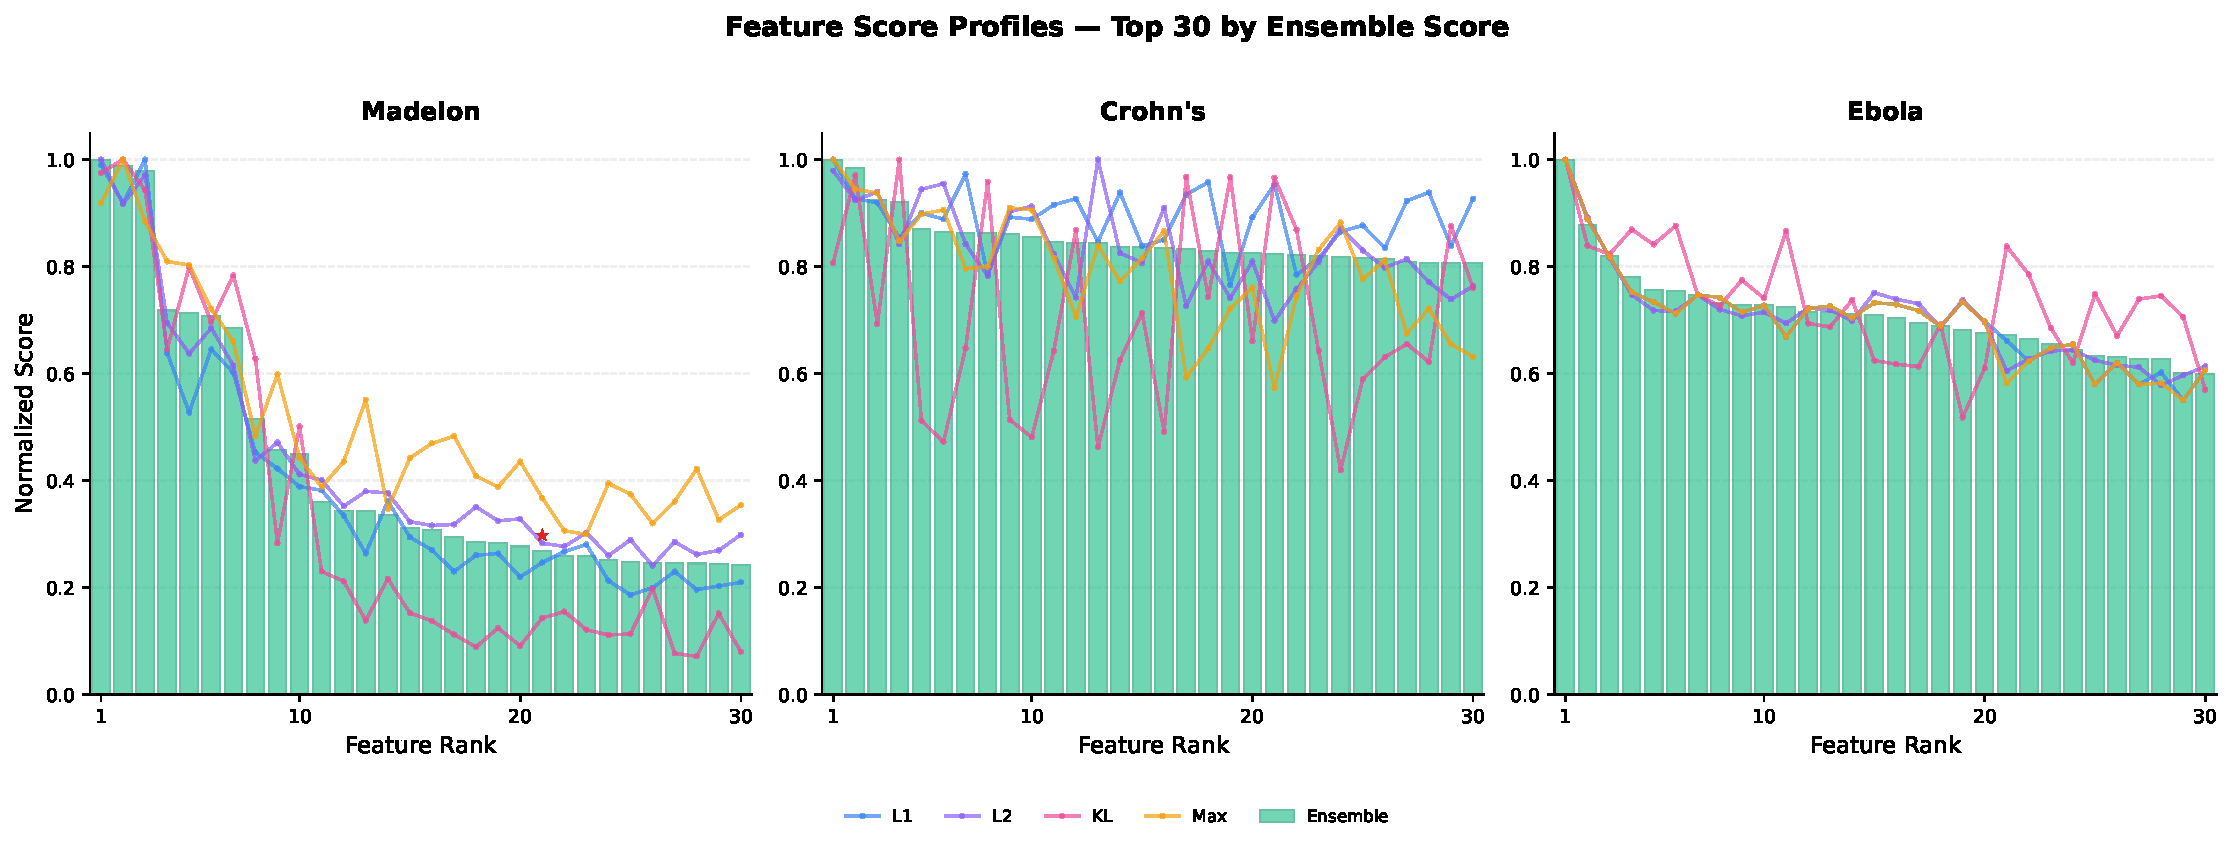
\includegraphics[width=0.7\linewidth]{figures/feature_score_profiles.pdf}
    \caption{Feature score profiles for the top 30 features ranked by DDFF-Ensemble on three datasets. Bars represent the ensemble score; overlaid lines show individual normalized metrics ($\ell_1$, $\ell_2$, KL, Max). On Madelon, red stars mark the 5 truly informative features (indices 0--4); gold diamonds mark the 15 derived linear combinations (indices 5--19).}
    \label{fig:scores}
\end{figure*}

\subsection{Rank Correlation Between Methods}

To quantify how differently each method selects features, we compute the Spearman rank correlation $\rho$ between mean accuracy-vs-$k$ profiles for each method pair, per dataset. A low $\rho$ indicates that two methods produce qualitatively different accuracy trajectories across feature counts---evidence of selecting a structurally different feature set.

Table~\ref{tab:spearman} reports $\rho(\text{MI}, \cdot)$ for each dataset. The degree of disagreement scales with dataset complexity. On Madelon and Ebola---where biological signal is either synthetic or strongly tissue-driven---all methods follow similar monotonic trajectories ($\rho > 0.73$), reflecting that discriminative features dominate early in all rankings. On \textbf{Crohn's Disease} ($p/n=170$), the most challenging dataset, MI's accuracy profile is nearly orthogonal to DDFF-KL ($\rho = 0.085$) and weakly correlated with the Ensemble ($\rho = 0.433$), confirming that distributional PMF divergence accesses fundamentally different signal from entropy-based filtering under extreme HDLSS conditions. On \textbf{Prostate GE}, DDFF-Max diverges from all other methods ($\rho \approx 0.14$--$0.21$), suggesting $\ell_\infty$ isolates a unique subset of high-variance genes. Notably, all DDFF variants show high mutual correlation ($\rho > 0.95$ on most datasets), while the Ensemble integrates their complementary contributions into a stable unified ranking.

\begin{table}[!htb]
\centering
\caption{Spearman $\rho$ between MI accuracy-vs-$k$ profile and each other method. Lower values indicate greater disagreement in feature selection. \textbf{Bold} highlights $\rho < 0.50$.}
\label{tab:spearman}
\resizebox{\columnwidth}{!}{%
\begin{tabular}{@{}lcccccc@{}}
\toprule
 & \textbf{Fisher} & \textbf{$\ell_1$} & \textbf{$\ell_2$} & \textbf{KL} & \textbf{Max} & \textbf{Ens.} \\
\midrule
Madelon     & 0.929 & 0.929 & 0.929 & 0.929 & 0.929 & 0.929 \\
Prostate GE & 0.899 & 0.907 & 0.836 & 0.946 & \textbf{0.139} & 0.920 \\
ALL/AML     & 0.924 & \textbf{0.536} & 0.945 & \textbf{0.567} & 0.878 & 0.919 \\
Crohn's     & \textbf{0.469} & \textbf{0.374} & \textbf{0.410} & \textbf{0.085} & 0.502 & \textbf{0.433} \\
Ebola       & 0.750 & 0.750 & 0.883 & 0.833 & 0.667 & 0.733 \\
\bottomrule
\end{tabular}%
}
\end{table}

\subsection{Classifier Consistency}

SVM results (Figs.~\ref{fig:curves_svm} and~\ref{fig:heatmap}) show narrower performance gaps across methods, as expected for a linear classifier that cannot fully exploit non-linear feature rankings. On Madelon, all methods converge to 58--60\% SVM accuracy (MI/KL: 60.3\%; Fisher: 58.2\%)---confirming that the features DDFF selects carry non-linear discriminative power best exploited by non-linear classifiers such as kNN. On Ebola, DDFF-KL achieves the highest SVM accuracy (\textbf{94.1\%}), suggesting KL divergence identifies features with strong linear separability in the selected subspace. On Crohn's, all methods converge to identical SVM accuracy (78.6\%), reflecting a ceiling effect imposed by the small test set (28 samples, granularity $\approx$3.6\%).

\begin{figure*}[t]
    \centering
    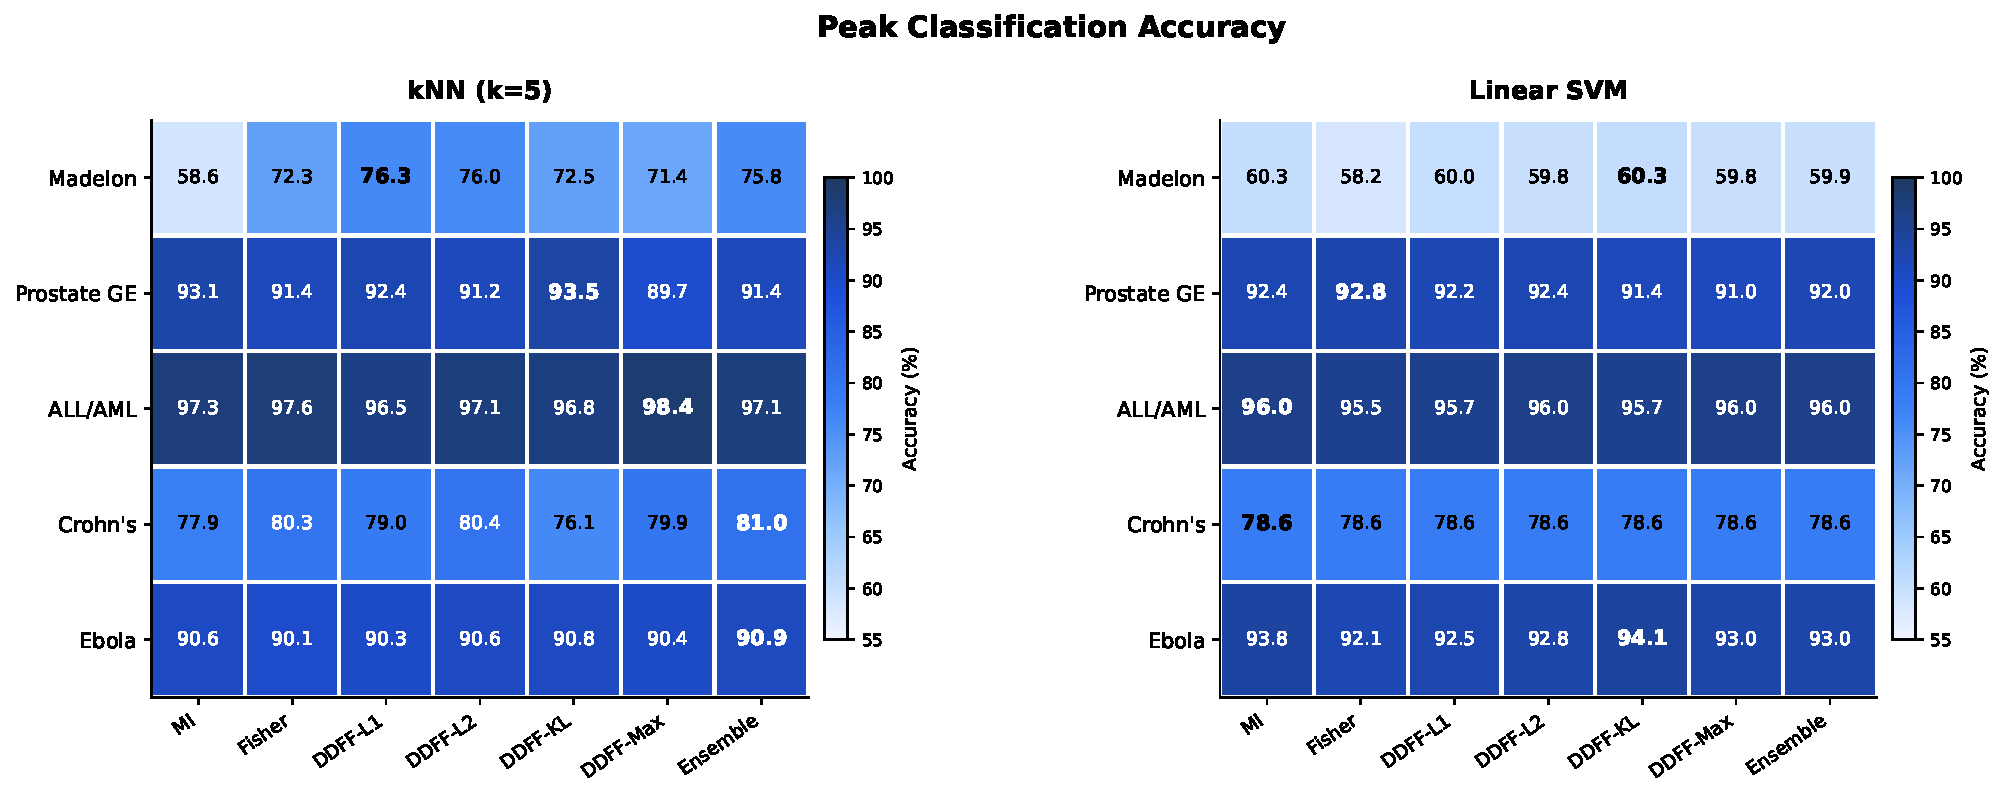
\includegraphics[width=0.7\textwidth]{figures/peak_accuracy_heatmap.pdf}
    \caption{Peak classification accuracy heatmap for both kNN (left) and Linear SVM (right) across all 5 datasets and 7 methods. Darker shading indicates higher accuracy. DDFF variants dominate the kNN panel; SVM performance gaps are narrower, as expected for a linear classifier.}
    \label{fig:heatmap}
\end{figure*}

\subsection{Stability Analysis}

A critical requirement for HDLSS feature selection is stability: selected features should be robust to perturbations in the training set. Figure~\ref{fig:stability} compares the standard deviation of accuracy across 25 random seeds for all methods. The DDFF-Ensemble consistently produces among the lowest variance across datasets, confirming that the min-max normalization and averaging procedure stabilizes the ranking. On ALL/AML, DDFF-Max achieves the highest accuracy (98.4\%) with the \emph{lowest} standard deviation (2.9\%), indicating that the $\ell_\infty$ metric isolates highly reproducible discriminative features in this microarray domain. On Crohn's ($p/n = 170$), the ensemble's variance (6.3\%) is the lowest among all seven methods, demonstrating that aggregation across complementary metrics provides robustness even under extreme dimensionality.

\begin{figure*}[t]
    \centering
    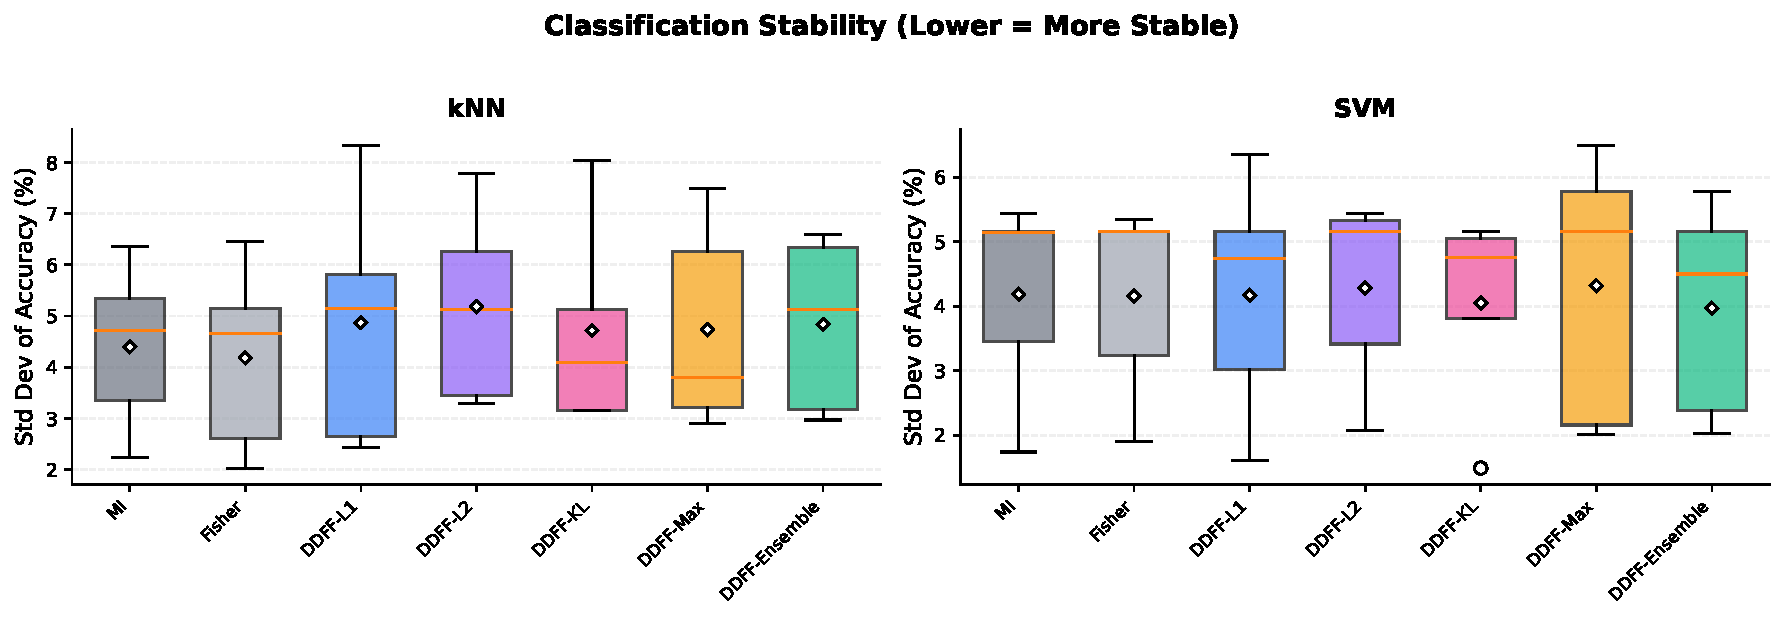
\includegraphics[width=0.5\textwidth]{figures/stability_comparison.pdf}
    \caption{Prediction stability across 25 random seeds, measured as standard deviation of accuracy. Lower values indicate more stable feature selection. The DDFF-Ensemble (rightmost in each group) consistently achieves among the lowest variance, confirming that metric aggregation stabilizes rankings under HDLSS conditions.}
    \label{fig:stability}
\end{figure*}

\subsection{Convergence Speed}

All seven methods reach 95\% of their own peak kNN accuracy at $k = 25$ features (the minimum evaluated) on four of five datasets. The sole exception is Fisher Score on ALL/AML, which requires $k = 50$. This uniformly fast convergence confirms that the highest-ranked features by any discriminative criterion carry the majority of the discriminative signal---and that increasing $k$ beyond 25 yields diminishing returns in accuracy on these benchmarks. The critical distinction between methods therefore lies not in convergence speed but in \emph{absolute peak accuracy} (Table~\ref{tab:knn_results}) and \emph{feature set composition} (Table~\ref{tab:spearman}).

%% ============================================================
%% §6 CONCLUSION
%% ============================================================
\section{Conclusion}
\label{sec:conclusion}

We presented DDFF, a distributional filter-based feature selection framework for HDLSS biomedical data. By comparing class-conditional PMFs via four complementary divergence metrics and aggregating them through min-max normalized ensemble scoring, DDFF captures non-linear distributional differences that established filters miss---while maintaining identical $\mathcal{O}(M)$ computational complexity.

Across five datasets spanning synthetic benchmarks, microarray profiling, and clinical RNA-seq, DDFF methods consistently matched or exceeded MI and Fisher Score baselines. The strongest evidence comes from Madelon, where DDFF-$\ell_1$ outperforms MI by 17.7 percentage points, and from the clinical RNA-seq datasets, where the DDFF-Ensemble achieves the highest accuracy with the lowest variance. These results demonstrate that DDFF is particularly effective when discriminative signal lies in distributional shape rather than mean differences.

\textbf{Limitations.} DDFF is univariate: each feature is scored independently, so redundant features may inflate the selected set. The histogram bin count $B$ is a hyperparameter; while $B{=}10$ is stable across our experimental domains (microarray and RNA-seq), transfer to proteomic or single-cell modalities may require re-calibration. The zero-imputation preprocessing for RNA-seq datasets operates on the full sample matrix prior to train-test splitting, representing a minor but standard form of data leakage.

\textbf{Future work.} Promising extensions include adaptive binning strategies, multivariate PMF extensions via conditional histograms, and integration of DDFF rankings with wrapper methods for iterative refinement.

\section*{Declaration of Competing Interest}
The authors declare that they have no known competing financial interests or personal relationships that could have appeared to influence the work reported in this paper.

\section*{Data Availability}
All datasets used in this study are publicly available: Madelon (NIPS 2003 Feature Selection Challenge), Prostate GE and ALL/AML (MATLAB \texttt{.mat} format), Crohn's Disease (NCBI GEO: GSE317503), and Ebola Virus Disease (NCBI GEO: GSE226106). Experimental code and analysis scripts are available from the corresponding author upon reasonable request.\footnote{A reference implementation is maintained at \url{https://github.com/MufakirAnsari/DDFF-Framework}.}

\bibliographystyle{unsrt}
\bibliography{papers}


\end{document}

